In this section, the characterization of uncladded BCF-12 fibers from Saint-Gobain, selected for the TRITIUM monitor, is described. These fibers are compared to single clad and multiclad BCF-12 fibers with the same external diameter to quantify the influence of the clad on their photon collection efficiency. Commercial clads are too thick ($30~\mu\meter$ for $1~\mm$ fiber diameter) for tritium measurements but a sufficiently thin clad could be obtained by vapor deposition if needed. The difference between these three types of fibers is that uncladded fibers consist of a polystyrene core with a refractive index of $1.60$, whereas single clad and multiclad fibers have a PMMA clad of $30~\mu\meter$ thickness and a refractive index of $1.49$. Multiclad fibers have, in addition, a second fluor-acrylic clad of $10~\mu\meter$ thickness and a refractive index of 1.42. The characterization was carried out for individual scintillating fibers and consisted in a comparative study of the fiber photon collection. The setup used, shown in Figure \ref{fig:SetUpFiberCharacterization}, consists of an optical board on which a LED and a PMT were placed in front of each other. A LED (LED435-03 from Roithner LaserTechnik Gmbh \cite{LEDRLT}), with an emission spectrum similar to that of the scintillating fibers, was used. The emission spectrum of the LED, given in Figure \ref{fig:LEDSpectrumTritium}, was measured using a spectrometer and fitted to a Gaussian function. The LED emission peak is at $434~\nano\meter$ with a $\sigma$ of $8~\nm$. The LED was fed in current mode with a sourcemeter. A calibrated Hamamatsu R8520-06SEL PMT with $QE=29.76\%$ quantum efficiency at $\lambda=430~\nano\meter$ was employed. 
\begin{figure}[h]
\centering
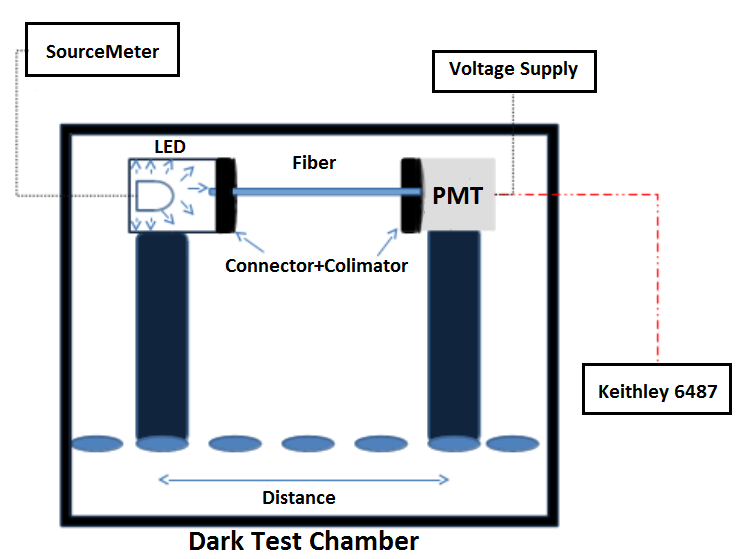
\includegraphics[scale=0.6]{4ResearchAndDevelopments/41Fibers/SetUp_Fiber_Characterization.png}
\caption{Setup used for fiber characterization.\label{fig:SetUpFiberCharacterization}}
\end{figure}
A $20~\cm$ long fiber was placed between the LED and the PMT, optically coupled to their end-surfaces by optical grease \cite{OpticalGrease}. Two collimators were used to ensure that only photons emitted from the LED were detected by the PMT. Two FH-ST connectors from RoHS \cite{} were used to fasten the fiber to the system. 
\begin{figure}[h]
\centering
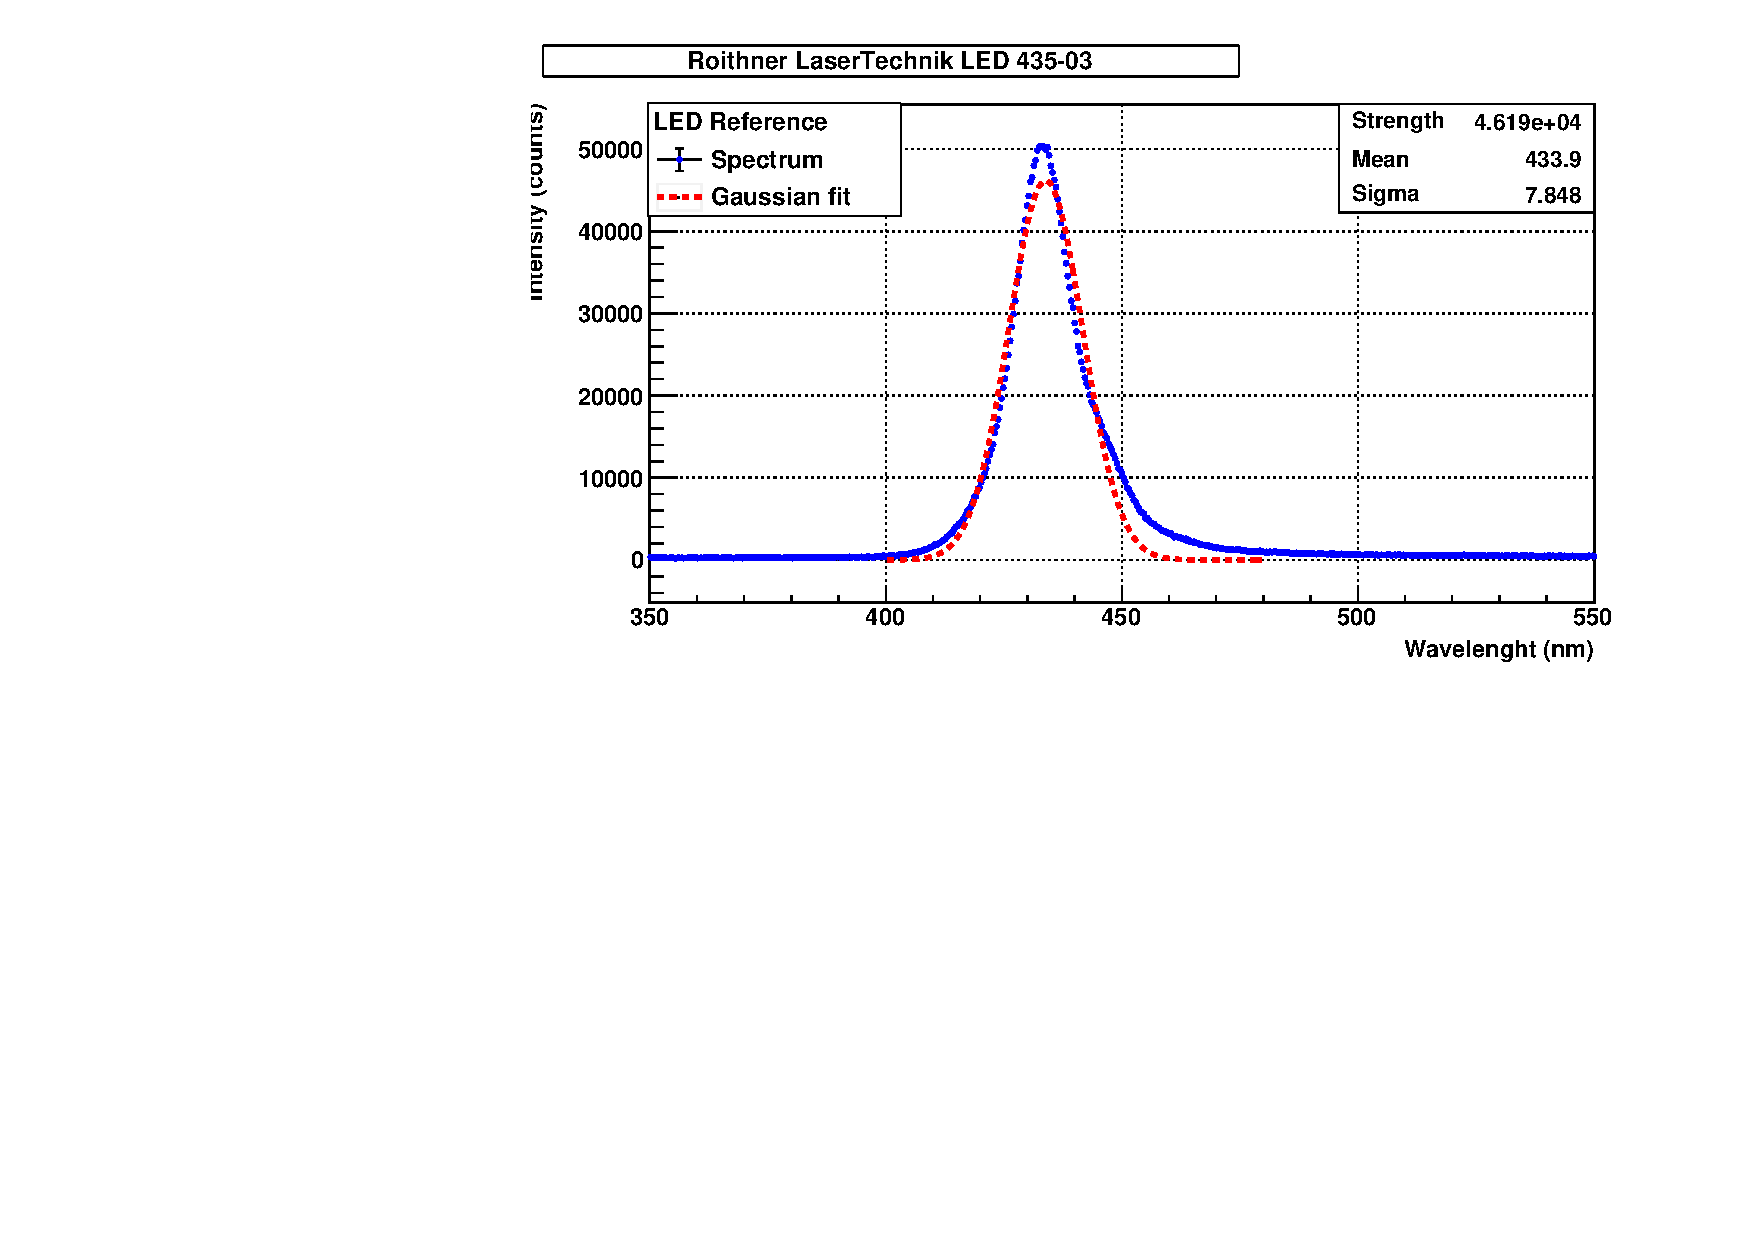
\includegraphics[scale=0.7]{4ResearchAndDevelopments/41Fibers/LED_TRITIUM_1_std.pdf}
\caption{Emission spectrum mesured for the 435-03 LED from Roithner LaserTechnik Gmbh.\label{fig:LEDSpectrumTritium}}
\end{figure}
To determine the photon collection efficiency, the rate of photons reaching the active area of the PMT was measured for the different type of fibers. The photon rate $R_{\gamma}$ reaching the photocathode was calculated from,
\begin{equation}
R_{\gamma} = \frac{\left( I_{PMT} - I_{DC} \right)}{q_e \cdot{} QE \cdot{} CE}
\label{eq:NumPhotonsFromIntensityPMT}
\end{equation}
where $I_{PMT}$ is the output current of the PMT, $I_{DC}$ is the dark current, $CE$ is the photoelectron collection efficiency and $q_e$ is the electron charge.